\documentclass[a4,11pt]{report} \usepackage[pdftex]{graphicx}
\usepackage{setspace}
\usepackage{lineno} \usepackage{color}
\definecolor{PiranaOrange}{rgb}{0.9,0.4,0.1}
\definecolor{Blue}{rgb}{0.0,0.0,0.7}
\definecolor{Red}{rgb}{0.7,0.0,0.0}
\definecolor{Grey}{rgb}{0.4,0.4,0.4}

\bibliographystyle{unsrt}%Choose a bibliograhpic style}
%\usepackage{utopia} %\usepackage{charter} %\usepackage{palatino}
%\usepackage{bookman} %\usepackage{newcent} %\usepackage{times}
%\usepackage[options]{natbib} \sloppy
\renewcommand{\familydefault}{\sfdefault} \oddsidemargin 1.5cm
\textwidth 14cm

\begin{document}

\title{\textbf{\textcolor{PiranaOrange}{Pira\~na: PCluster}}\\ \vspace{15pt}

\includegraphics[scale=0.12]{images/pirana_logo.jpg} \\ \vspace{15pt}
\scriptsize Installation guide and Manual \\
\vspace{5pt} \scriptsize {\today} \\
\date{}}
\maketitle

\tableofcontents

\chapter{PCluster} The \textcolor{Blue}{PCluster} system is aimed to
be a system for distributed NONMEM computing for smaller modeling
groups, e.g. in hospital or academic settings. If budget poses no
problems, other cluster solutions are probably more adequate. Our major development goal
was to develop a system that could be installed on an existing
(Windows-based) network, and that would use spare CPU cycles of
non-dedicated PCs in the network.

\section{Description and requirements} The infrastructure uses
PC's in a standard Windows network environment, which can e.g. be PC's
dedicated to running NONMEM, or PC's of co-workers, or a combination
of both. The PCluster can be set up without the need for vast
hardware/software knowledge. Distribution to multi-core CPU's is
possible, and tested up to a total of 40 CPUs.

The infrastructure requires a shared network-drive accessible by all
clients (standard desktop PC's in a network environment). On this
shared network drive, a version of Perl and Fortran must be
present. Furthermore, the PCluster \textit{daemon} Perl-script
needs to run in the background on each node. On
the client computer, i.e. the modeler's computer, Pira\~na needs to be
installed. Below, more information is provided on how to set this up.

\section{Installation} First, it is necessary to reserve up some
harddisk space on your network, to be accessible (read and write) by
all clients, mounted as a drive on all nodes (let's assume this to be
U:). Copy the contents of the folder
\ttfamily{\/install\_on\_each\_node} \normalfont in the
\ttfamily{/cluster} \normalfont folder in the Pira\~na home folder to
this drive. Next, the daemon script (or the compiled version of it) should be
installed and running on each client in the network. For this, copy
the folder $\backslash$pcluster$\backslash$install\_on\_each\_node located in the Pirana home folder in the
harddisk root (C:$\backslash$). The daemon can be started manually by
executing the Perl script daemon.pl or the daemon.exe.  Before
starting, check the settings in
C:$\backslash$pcluster$\backslash$pcluster.ini. This file contains the
info for the client, e.g. the number of CPUs to use, and how to
connect to the shared drive.  Instead of starting the daemon manually, it is recommend to run the daemon as Windows service, which has the advantage that users are able to log in and out without compromising the integrity of the PCluster, and that
the service is automatically started when the PC is started. To
install this service, run the Perl script inst\_daemon.pl:
\begin{verbatim} perl inst_daemon.pl
\end{verbatim} This will create the information in the Windows
registry for the PDaemon service. If no error is reported, the service
can now be started from the command line with:
\begin{verbatim} NET START PDaemon
\end{verbatim}

It has been reported that the daemon sometimes isn't working properly
(i.e. not requesting PsN/nfme runs), while the script \'is working
properly when it is run manually. Running the daemon manually is
however a problem, as a console window will appear each time a run is
processing, which is annoying to the principal user of the machine. A
workaround for this is to download a tool called CMDOW (available from
http://www.commandline.co.uk/cmdow/). If you start the following
command (e.g. in a batch script at startup), no consoles will appear:
\begin{verbatim} u:\cmdow.exe /run /hid u:\perl\bin\perl.exe c:\pcluster\pdaemon.pl
\end{verbatim}

\vspace{8pt}
\noindent\scriptsize{\textcolor{Blue}{Note:} \textcolor{Grey}{Thanks
to Andreas Lindauer for suggesting this workaround.  } \normalsize


\subsection*{Perl and PsN} Make sure Perl (with
PsN installed) is available on the cluster-drive (e.g. in
U:$\backslash$Perl). Also check that you have the following Perl
modules installed: LockFile, Sys::Hostname and File.  Since this
option hasn't been fully developed yet in PsN, it is necessary to make
a few changes in some PsN source files (using PsN 3.1.0 as a
template).
\begin{itemize}
\item In \textcolor{Blue}{nonmem.pm} in the PsN directory, add the
following lines at the top of the source-file:
\begin{verbatim}
my $fortran_dir = 'U:\MinGW\bin';
unless ($ENV{'PATH'} =~ m/$fortran_dir/) {
  $ENV{'PATH'} = $fortran_dir.";".$ENV{'PATH'};
}
\end{verbatim} This ensures the Fortran compiler is in the path
(change U:$\backslash$MinGW$\backslash$bin' to the fortran path that
you use). Of course this is not necessary if this directory is
already permanently in the PATH environment variable.

\item In \textcolor{Blue}{tool$\backslash$modelfit.pm} change line
3014:
\begin{verbatim}
  require File::Temp; # qw/tempfile tempdir/;
  require Sys::Hostname;
  require LockFile::Simple; # qw/lock unlock trylock/; #Non-standard module
\end{verbatim}
into
\begin{verbatim}
  use File::Temp qw/tempfile tempdir/;
  use Sys::Hostname;
  use LockFile::Simple qw/lock unlock trylock/;  # Non-standard module
  use File::Basename;
\end{verbatim}

In the same file, move the contents of line 3063:
\begin{verbatim}
  return $jobId;
\end{verbatim}
to line 3057, just after the line with `unlock \$jobId;'.

In the same file, around line 3105, change:
\begin{verbatim}
  if( -e "$ZinkDoneDir$jobId" ){
\end{verbatim}
into
\begin{verbatim}
  use File::Basename;
  my $job = basename($jobId);
  if( -e "$ZinkDoneDir/$job" ){
\end{verbatim}

\item In psn.conf file in the PsN folder on the cluster, edit the
following lines with your settings (also remove leading semi-colons):
\begin{verbatim}
40 : perl = U:\Perl\bin\perl.exe
82 : zink_dir = U:
105: default=U:\nmvi,6
\end{verbatim} Of course, the other PsN settings should be set correctly as well.

\end{itemize}

\subsection*{Fortran (g77)} If you want to use the PsN-toolkit on
the PCluster, you must provide access to a Fortran compiler for each
client in the cluster. This is because PsN runs are compiled after
distribution to a client. If you only make use of Pirana's own
distribution capabilities, only a Fortran compiler on the modeler's
own computer is required. The recommended way is to use a central
installation of Fortran on the cluster drive, e.g. g77 supplied with
MinGW. For this, e.g. install MinGW with g77 on your local
computer. After installation, copy the folder MinGW to the cluster
drive.

\subsection*{Pirana preferences} In Pira\~na the following
preferences should be updated:
\begin{description}
	\item \textcolor{Grey}{zink\_host}:
e.g. \textcolor{Blue}{ZinkHost}, A host name for the Zink / PCluster,
should correspond with the hostname specified in psn.conf.
\end{description}
\noindent And in `software settings', change:
\begin{description}
  \item \textcolor{Grey}{f77\_dir}: Path to Fortran on the
cluster-drive e.g.  \textcolor{Blue}{U:/MinGW/bin}
  \item \textcolor{Grey}{perl\_dir}: Path to Perl on the cluster-drive
e.g.  \textcolor{Blue}{U:/Perl}
  \item \textcolor{Grey}{psn\_dir}: Path to PsN on the cluster-drive
e.g.  \textcolor{Blue}{U:/Perl/site/lib/PsN\_2\_3\_1}
\end{description}

\subsection*{Troubleshooting} The PCluster, although it functions
quite adequately in the current setup, is actually still in beta
phase. If you have questions regarding the set-up or functionality of
the PCluster, please send a mail to the mailinglist
(\textcolor{Grey}{info@pirana-software.com}) or contact the
Pira\~na development team directly.

\pagebreak
\section{Working with the PCluster}

\subsection*{Using the PsN toolkit on PCluster} This functionality
is enabled by specifying `-run\_on\_zink' on the PsN command line from
the Pira\~na window, after selecting a PsN tool from the toolkit. You
should leave the PsN console window open until the run is finished,
since the instance of PsN that is running locally will take care of
the run distribution and calculation and formatting of data files
after finishing the cluster run(s).

\subsection*{Cluster monitor} Using the cluster monitor (`View
$\rightarrow$ Cluster monitor') the activity and availability of
clients can be monitored. Note that status of the client might take a
half a minute to refresh with the up-to-date information, due to the
interval used by the daemon-script.  \vspace{10pt}

\begin{figure}[hbt] \centering
    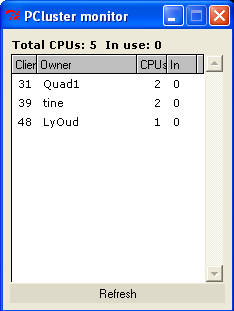
\includegraphics[scale=0.5]{images/pcluster.png}
    \caption{PCluster monitor}
\end{figure}


\end{document}